\subsection{積分定理}
	
	本稿では,複素数$z$と$w$に対して
	\begin{align}
		[0,1] \ni t \longmapsto z + t \cdot (w - z)
	\end{align}
	なる写像を
	\begin{align}
		\seg{z}{w}
	\end{align}
	と表す.つまり
	\begin{align}
		\seg{z}{w} \defeq \Set{(t,\zeta)}{t \in [0,1] \wedge \zeta = z + t \cdot (w - z)}
	\end{align}
	と定める.$\seg{z}{w}$とは$z$から$w$に直進する線分を描き,また$f$を$\seg{z}{w}$上の連続写像とすれば
	\begin{align}
		\int_{\seg{z}{w}} f = (w-z) \cdot \int_{[0,1]} f(z + t \cdot (w - z))\ dt
	\end{align}
	が成り立つ.また$t$を$[0,1]$の要素とすれば
	\begin{align}
		\seg{w}{z}(t) = \seg{z}{w}(1 - t)
	\end{align}
	が成り立つので,$\seg{w}{z}$は$\seg{z}{w}$の逆路である.ゆえに
	\begin{align}
		\int_{\seg{w}{z}} f = - \int_{\seg{z}{w}} f
	\end{align}
	が成立する.
	
	いま$a$と$b$と$c$を複素数とすると,
	\begin{align}
		\Delta \defeq \Set{z}{\exists t,s \in [0,1]\, 
		\left(\, z = (1-t) \cdot a 
		+ t \cdot (1-s) \cdot b 
		+ t \cdot s \cdot c\, \right)}
	\end{align}
	により定める集合$\Delta$は,イメージとしては$a,b,c$によって囲まれる三角形
	
	\begin{center}
	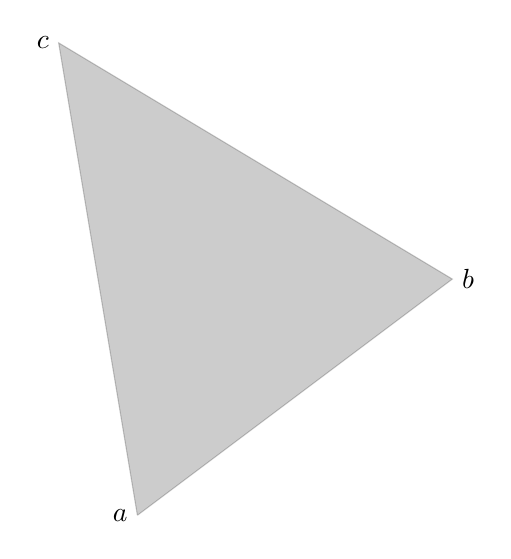
\begin{tikzpicture}
		\filldraw[opacity=0.2] (0,0)--(4,3)--(-1,6)--(0,0);
		\node[anchor=east] at (0,0) {$a$};
		\node[anchor=west] at (4,3) {$b$};
		\node[anchor=east] at (-1,6) {$c$};
	\end{tikzpicture}
	\end{center}
	
	を表す.この$\Delta$は$\C$のコンパクト部分集合である.実際,
	\begin{align}
		(t,s) \longmapsto (1-t) \cdot a + t \cdot (1-s) \cdot b + t \cdot s \cdot c
	\end{align}
	は$\R^2$から$\C$への連続写像であって,$\Delta$とはこの写像によって
	\begin{align}
		[0,1] \times [0,1]
	\end{align}
	なる$\R^2$のコンパクト部分集合を写した像である.
	
	三角領域の外郭に沿った正則関数の線積分は$0$になる.
	
	\begin{screen}
		\begin{thm}[Cauchy-Goursatの定理]
			$a$と$b$と$c$を複素数とし,
			\begin{align}
				\Delta \defeq \Set{z}{\exists t,s \in [0,1]\, 
				\left(\, z = (1-t) \cdot a 
				+ t \cdot (1-s) \cdot b 
				+ t \cdot s \cdot c\, \right)}
			\end{align}
			と定める.また$\Omega$を$\Delta$を含む$\C$の開集合とし,
			$f$を$\Omega$上の$\C$値連続写像とし,$p$を$\Omega$の要素とする.
			このとき,
			\begin{align}
				f \in H(\Omega \backslash \{p\})
			\end{align}
			であれば
			\begin{align}
				\int_{\seg{a}{b}} f + \int_{\seg{b}{c}} f + \int_{\seg{c}{a}} f = 0
			\end{align}
			が成立する.
		\end{thm}
	\end{screen}
	
	\begin{screen}
		\begin{thm}[凸開集合に含まれる任意の三角形の周上の積分が$0$である連続写像は正則関数の導関数]
			$\Omega$を$\C$の凸開集合とし,$f$を$\Omega$上の$\C$値連続写像とする.
			このとき,$\Omega$の任意の三要素$a$と$b$と$c$に対して
			\begin{align}
				\int_{\seg{a}{b}} f + \int_{\seg{b}{c}} f + \int_{\seg{c}{a}} f = 0
			\end{align}
			が満たされているならば,$p$を$\Omega$の要素として$F$を
			\begin{align}
				\Omega \ni z \longmapsto \int_{\seg{p}{z}} f
			\end{align}
			なる関係により定める写像とすれば
			\begin{align}
				F' = f
			\end{align}
			が成立する.
		\end{thm}
	\end{screen}
	
	\begin{sketch}
		$\Omega$の任意の三要素$a$と$b$と$c$に対して
		\begin{align}
			\int_{\seg{a}{b}} f + \int_{\seg{b}{c}} f + \int_{\seg{c}{a}} f = 0
		\end{align}
		が満たされているとする.また$p$を$\Omega$の要素として,
		\begin{align}
			\Omega \ni z \longmapsto \int_{\seg{p}{z}} f
		\end{align}
		なる写像を$F$とする.$z$と$w$を$\Omega$の要素とすれば
		\begin{align}
			\int_{\seg{z}{w}} f = -\int_{\seg{w}{p}} f - \int_{\seg{z}{p}} f
		\end{align}
		が成り立つが,
		\begin{align}
			\int_{\seg{w}{p}} f = -\int_{\seg{p}{w}} f = -F(w)
		\end{align}
		より
		\begin{align}
			\int_{\seg{z}{w}} f = F(w) - F(z)
		\end{align}
		が得られる.よって,$h$を
		\begin{align}
			z + h \in \Omega
		\end{align}
		である範囲の任意の複素数とすれば
		\begin{align}
			F(z+h) - F(z) - h \cdot f(z)
			&= \int_{\seg{z}{z+h}} f - h \cdot f(z) \\
			&= h \cdot \int_{[0,1]} f(z + t \cdot h) - f(z)\ dt
		\end{align}
		が成立する.ところで$f$は$z$で連続であるから,いま$\epsilon$を任意に与えられた正の実数とすれば
		\begin{align}
			|h| < \delta \Longrightarrow |f(z+h) - f(z)| < \epsilon
		\end{align}
		を満たす正の実数$\delta$が取れる.そして$h$を
		\begin{align}
			|h| < \delta
		\end{align}
		を満たす任意の複素数とすれば
		\begin{align}
			|F(z+h) - F(z) - h \cdot f(z)|
			\leq |h| \cdot \int_{[0,1]} |f(z + t \cdot h) - f(z)|\ dt
			< |h| \cdot \epsilon
		\end{align}
		が成り立つ.ゆえに$F$は$z$で微分可能であり,その微分係数は
		\begin{align}
			f(z)
		\end{align}
		である.
		\QED
	\end{sketch}